\documentclass{standalone}

\usepackage{tikz}
\usetikzlibrary{calc,shapes.multipart,chains,arrows,positioning}
\tikzset{
    squarecross/.style={
        draw, rectangle,minimum size=18pt, fill=orange!80,
        inner sep=0pt, text=black,
        path picture = {
            \draw[black]
            (path picture bounding box.north west) -- 
            (path picture bounding box.south east)
            (path picture bounding box.south west) -- 
            (path picture bounding box.north east);
        }
    }
}

\begin{document}
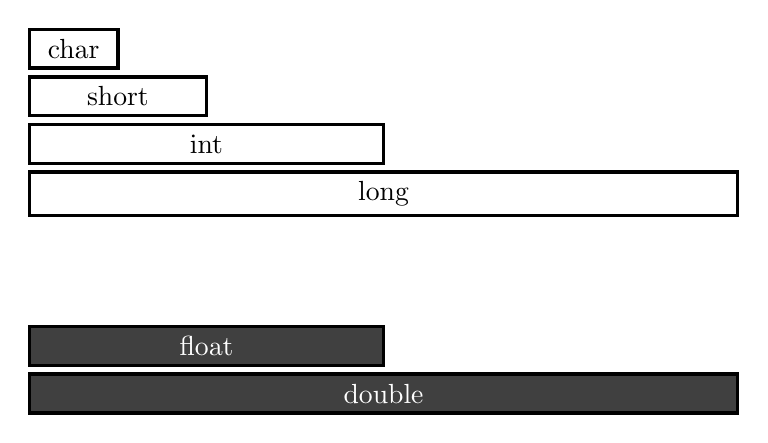
\begin{tikzpicture}[
        list/.style={
            very thick, rectangle split, 
            rectangle split parts=3, draw, 
            minimum size=18pt,
            inner sep=5pt, text=black,
            rectangle split part fill={blue!20, red!20, blue!20}
        }, 
        ->, start chain, very thick
      ]


  \node   (char) [minimum width=32pt,minimum height=14pt,draw] {char};
  \node   (short) [below=2pt of char.south west,anchor=north west,minimum width=64pt,minimum height=14pt,draw] {short};
  \node   (int) [below=2pt of short.south west,anchor=north west,minimum width=128pt,minimum height=14pt,draw] {int};
  \node   (long) [below=2pt of int.south west,anchor=north west,minimum width=256pt,minimum height=14pt,draw] {long};


  \node   (float) [below=75pt of short.south west,anchor=north west,minimum width=128pt,minimum height=14pt,draw,fill=darkgray,text=white] {float};
  \node   (double) [below=2pt of float.south west,anchor=north west,minimum width=256pt,minimum height=14pt,draw,fill=darkgray,text=white] {double};


\end{tikzpicture}
\end{document}